\section{Panoramica}
GameUp è un software dedicato a due tipi di utenti finali: videogiocatori e sviluppatori di videogiochi. Il sistema deve offrire un insieme di funzionalità base per tutti gli utenti, oltre che a funzionalità specifiche per le singole specializzazioni.
In particolare, le funzionalità base da offrire sono:
\begin{itemize}
\item Mostrare un catalogo di videogiochi attualmente attivi nella piattaforma, mostrando delle informazioni di base ed offrendo dettagli aggiuntivi come descrizione, immagini di esempio e recensioni al click dell’utente;
\item Permettere l’acquisto di un videogioco dalla pagina del dettaglio di esso;
\item Permettere funzionalità di autenticazione (registrazione e log-in) per rendere più semplice l’interazione con la piattaforma, salvando il metodo di pagamento o permettendo la stesura di una recensione, o di avere accesso a funzionalità dedicate agli sviluppatori o agli amministratori;
\item Filtrare il catalogo per trovare giochi inerenti ai gusti dell’utente, o per rimuovere giochi indesiderati;
\end{itemize}
Mentre le funzionalità aggiuntive dedicate agli sviluppatori sono:
\begin{itemize}
\item Richiedere l’aggiunta del proprio videogioco all’interno della piattaforma compilando un modulo contenente le informazioni necessarie;
\item Gestire i propri videogiochi pubblicati, modificandone le informazioni;
\item Gestire il forum dedicato al proprio videogioco, dando la possibilità di creare una comunità affiatata e di rispondere ad eventuali domande poste dagli utenti;
\end{itemize}
Infine, le funzionalità aggiuntive degli amministratori della piattaforma sono:
\begin{itemize}
\item Avere il controllo totale della piattaforma, potendo quindi modificare le informazioni di qualsiasi videogioco, per poter moderare le informazioni dove necessario;
\item Approvare o negare le richieste di inserimento di videogiochi da parte degli sviluppatori;
\item Gestire eventuali problemi sotto forma di ticket da parte degli utenti;
\item Poter moderare le comunità dei vari videogiochi, in particolare potendo cancellare eventuali messaggi o recensioni con contenuti dannosi, come ad esempio lo spam;
\end{itemize}

\section{Identificazione degli attori}
\begin{center}
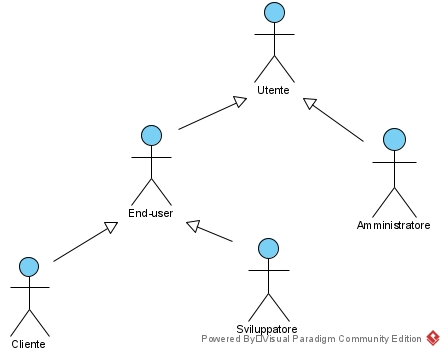
\includegraphics{Figure/actorsDiagram.jpg}
\end{center}

\section{Requisiti funzionali}
\subsection{RF Gestione Account (Utenti)}
\begin{enumerate}
	\item \textbf{Registrazione}: Un utente non registrato deve poter registrarsi alla piattaforma;
	\item \textbf{Log-in}: L’utente registrato deve poter immettere le sue credenziali per potersi autenticare;
	\item \textbf{Logout}: L’utente autenticato deve poter uscire dalla piattaforma;
	\item \textbf{Visualizza profilo}: L’utente autenticato deve poter visualizzare le informazioni collegate al suo account;
	\item \textbf{Modifica Profilo}: L’utente autenticato deve poter modificare le informazioni relative al suo account. In particolare, deve poter segnare l’opzione Sviluppatore per diventare uno Sviluppatore;
	\item \textbf{Recupera Password}: L’utente registrato deve poter richiedere il reset della password nel caso se ne sia dimenticato;
	\item \textbf{Chiusura Discussione}: Un utente deve poter essere in grado di chiudere una discussione, la propria se è un cliente, una relativa al proprio videogioco se è uno sviluppatore oppure tutte nel caso di un amministratore.
\end{enumerate}

\subsection{RF End-user}
\begin{enumerate}
	\item \textbf{Creazione Discussione}: Un end-user deve poter creare una discussione all’interno del forum dedicato ad un particolare videogioco.
	\item \textbf{Commento Discussione}: Un end-user deve poter commentare in una discussione esistente, nel caso non sia chiusa.
	\item \textbf{Visualizzazione Comunità Videogioco}: Il visitatore deve poter visualizzare il forum dedicato ad un determinato videogioco, formato da discussioni contenenti messaggi scritti da utenti autenticati, in particolare dagli autori del videogioco;
\end{enumerate}

\subsection{RF Clienti}
\begin{enumerate}
	\item \textbf{Visualizzazione Pagina Iniziale}: Il cliente deve poter visualizzare una vetrina di videogiochi selezionati secondo vari criteri dal sistema;
	\item \textbf{Visualizzazione Catalogo}: Il cliente deve poter visualizzare il catalogo di tutti i videogiochi attivi della piattaforma, ovvero i dettagli sostanziali che lo descrivono come nome, prezzo, autore e logo, avendo la possibilità di filtrarli secondo determinati criteri;
	\item \textbf{Visualizzazione Dettagli Videogioco}: Il cliente deve poter visualizzare i dettagli relativi ad un particolare videogioco, come ad esempio la descrizione per esteso, la versione, immagini di anteprima e le recensioni;
	\item \textbf{Acquisto Videogioco}: Il cliente autenticato deve poter effettuare il download del gioco scelto dalla sua schermata dei dettagli, nel caso sia gratis, oppure previo pagamento. In particolare, deve poter avere la possibilità di scegliere la versione da scaricare;
	\item \textbf{Recensione Videogioco}: se lo consiglierebbe ad un amico ed eventuali note aggiuntive lasciate come testo;
	\item \textbf{Valutazione Recensione}: Il cliente autenticato deve poter valutare una singola recensione in maniera positiva o negativa.
	\item \textbf{Suggerimento Tags}: Il cliente autenticato deve poter suggerire ulteriori tag per un videogioco acquistato, scegliendone una tra le più popolari del momento oppure fornendo una propria tag come suggerimento.	
\end{enumerate}

\subsection{RF Sviluppatori}
\begin{enumerate}
	\item \textbf{Richiesta Inserimento Videogioco}: Lo sviluppatore deve poter accedere ad un modulo compilabile, tramite il quale può richiedere agli amministratori della piattaforma la pubblicazione del proprio videogioco;
	\item \textbf{Messa in Rilievo di una Discussione}: Lo sviluppatore deve poter fissare come discussione importante una o più discussioni contenute all’interno del forum dedicato ad un videogioco pubblicato da lui.
	\item \textbf{Richiesta di Modifica Dati Videogioco}: Lo sviluppatore deve poter modificare le informazioni relative ad un gioco da lui pubblicato. In particolare, deve poter caricare una nuova versione del suo videogioco (un aggiornamento), senza però sovrascrivere le versioni esistenti, le quali rimangono pubbliche e scaricabili.
	\item \textbf{Sponsorizzazione Videogioco}: Lo sviluppatore deve poter sponsorizzare un proprio videogioco, specificando le settimane durante le quali applicare i privilegi della sponsorizzazione, tra quelle mostrate come disponibili dal sistema previo pagamento.	
\end{enumerate}

\subsection{RF Amministratori}
\begin{enumerate}
	\item \textbf{Risoluzione richieste pubblicazione/modifica videogiochi}: L’amministratore deve poter accettare o rifiutare una richiesta di pubblicazione o di modifica di un videogioco.
	\\Nel caso di una approvazione, il sistema provvede a creare e rendere pubblica la schermata di dettaglio del videogioco basandosi sui dati forniti dallo sviluppatore nel modulo da lui pubblicato.
	\item \textbf{Modifica dati videogioco}: L’amministratore deve poter modificare immediatamente i dati relativi ad un videogioco, direttamente dalla pagina dei dettagli di tale, senza dover richiedere l’approvazione di un altro amministratore.
	\item \textbf{Rimozione contenuto offensivo}: L’amministratore deve poter nascondere contenuti pubblici di qualsiasi tipo, come ad esempio videogiochi, commenti o discussioni nocive e recensioni per il bene della piattaforma;
	\item \textbf{Risoluzione report}: L’amministratore deve poter marcare un report come risolto, sia in maniera positiva oppure negativa, così che il sistema possa avvisare automaticamente gli utenti relativi ad un determinato report delle azioni eseguite dall’amministratore per la risoluzione.	
\end{enumerate}

\section{Requisiti non funzionali}
\subsection{Usabilità}
Il sistema deve essere accessibile da qualsiasi piattaforma, in particolare per i dispositivi mobile, ovvero i target principali del sistema. Opzionalmente, deve essere accessibile anche da dispositivi non mobile, come ad esempio un desktop, principalmente per rendere più semplice l’uso per gli sviluppatori e gli amministratori. I contenuti caricati dagli sviluppatori devono seguire un format standard, così da non confondere gli utenti durante la navigazione del catalogo.

\subsection{Affidabilità}
Il sottosistema di autenticazione degli utenti registrati deve essere robusto, basandosi su un algoritmo di sicurezza valido e gli utenti devono avere accesso solo specificatamente alle risorse necessarie, nella modalità necessaria (solo lettura o lettura e scrittura). Gli sviluppatori devono avere più permessi di un normale utente registrato, ma solo per le pagine relative ai loro videogiochi, senza poter impersonare o abusare, però, altri utenti o altri videogiochi, ad esempio nel forum non devono poter cancellare i contenuti altrui, per evitare la cancellazione di feedback negativi validi, mentre le richieste di aggiunta o modifica del proprio videogioco devono necessariamente passare per un controllo di validazione da parte degli amministratori, per evitare contenuti atti a danneggiare la piattaforma.

\subsection{Performance}
Il sistema deve poter soddisfare le richieste di svariati utenti, utilizzando servizi moderni per la distribuzione di contenuti. In particolare, il download e l’upload dei videogiochi non devono impattare la visualizzazione del sito, essendo l’operazione più onerosa del sistema.

\subsection{Manutenibilità}
Il sistema deve essere dotato dei test necessari per garantire, in primis, che la parte dedicata agli utenti finali non subisca danni durante gli aggiornamenti del sistema, per evitare aggiornamenti dannosi.

\subsection{Legali}
I dati personali degli utenti registrati devono essere trattati secondo le regole definite dal Regolamento Ue 2016/679, noto come GDPR. La cancellazione di un videogioco dal sistema da parte degli amministratori deve essere possibile nel caso di problemi legali derivanti da quel videogioco, ad esempio se uno sviluppatore pubblica un videogioco non realizzato da lui. Inoltre, i pagamenti all’interno della piattaforma vengono processati con un servizio esterno, per garantire la sicurezza dei dati, per poi essere divisi con i singoli sviluppatori mantenendo una determinata percentuale pattuita dal contratto firmato dalla società del sistema GameUp e lo sviluppatore di un videogioco inserito. 

\section{Modello del sistema}
\subsection{Scenari}
\begin{center}
	\begin{tabular}{|| m{2em} | m{8em} ||} 
	\hline
	Col1 & Col2
	\hline\hline
	1 & 6
	\hline
	2 & 7
	\hline
	3 & 545
	\hline
	4 & 545
	\hline
   \end{tabular}
   \end{center}